\section{Design and the \textit{open-closed-principle}}
One main purpose of the use of java and object-oriented programming is that the code is easily
extended so new features and functions can easily be added to an already working system.
Nevertheless, one has to respect some rules of programming in order to benefit from this advantage,
i.e. the use of design patterns.
In our \textit{MyFoodora} we used several of these patters which are explained in this section.

\subsection{Package Management}
\label{sub:package_management}

Having read the project requirements for the first time we figured out that there were several
different parts which can be treated seperately. This logic sepration of different parts of the
system was used to organize our packages as well as the division of the work for the two members of
the group. The following main packages exist in the project:
\begin{itemize}
	\item{\textbf{system}} Contains the main funtionalities of \textit{MyFoodora}.
	\item{\textbf{user-management}} Manages users of the systems and asseses functions
		to groups of users.
	\item{\textbf{restaurant}} Manages the creation of meals and singleItems and do the pricing.
	\item{\textbf{commandLineTool}} Adds a command line user interface to the system.
	\item{\textbf{GUI}} Adds a graphical user interface to the system.
	\item{\textbf{several Test packages}} According their name they provide test for the
		previous packages.
\end{itemize}

The following diagram shows the interaction of the first three packages (The interfaces and testings 
do obviously interact with all the other ones).

\begin{figure}[H]
	\centering
	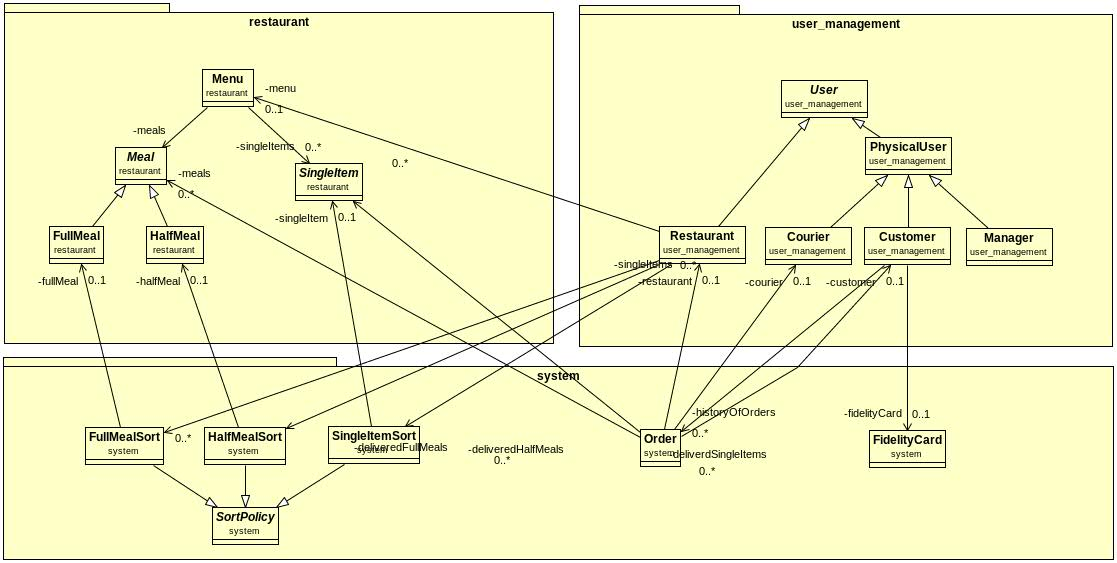
\includegraphics[width=1\linewidth]{./ima/packages.jpg}
	\caption{Package-interactions, class \textit{MyFoodora} excluded to simplify}
	\label{fig:packages}
\end{figure}

The graphic \ref{fig:packages} shows the three main packages that form the core of our system. All
interaction between the packages are displayed except from those with the class \textit{MyFoodora}.
The seperation choosen allowed us to seperately work on the \textsc{user-management} and
\textsc{restaurant} without depending on parts of the code of the other package, because there is 
only one interaction between the two. In a third stey we implemented \textsc{system}, because it was
the most sophisticated one and requires large parts of the two other packages. \textit{Order} is the most connected class besides \textit{MyFoodora}. One might consider to place it in a of the other 
packages. We decided to store it in the system because we wanted functions like the computation of 
an order's price to be part of the system. In this manner we were able to keey all the core functions
together. 

\subsection{DesignPattern Factory-Pattern}
\label{sub:designpattern_factory_pattern}

A major pattern to respect the \textit{open-closed-principle} is the Factory-Pattern because it
allows the code to be easily extended without modifying the existing code. It is used twice in the
system:
\begin{enumerate}
	\item Creation of Items for the Restaurant
	\item Creation of Users in the user-management
\end{enumerate}
